\documentclass[]{article}
\newcommand{\FileDepth}{../../..}
\usepackage[letterpaper, landscape, margin=0.5cm]{geometry}
\usepackage[T1]{fontenc}
\usepackage{textcomp}%Not strictly necessary, but gives \textmu command for "micro."
\usepackage{fancyhdr}
\usepackage{amsmath}
\usepackage{amssymb}
\usepackage{graphicx}
\usepackage{xcolor}
\usepackage{tikz}
\usetikzlibrary{calc}
\usepackage[shortlabels]{enumitem}
\usepackage{multicol}
\usepackage{vwcol}
\usepackage{hyperref}
\usepackage{wrapfig}
%opening
\newcommand{\SecType}{L}
\newcommand{\Week}{11}
\title{PH 211 Lecture \Week}
\author{Benjamin Bauml}
\date{Summer 2024}

\newcommand{\Purpose}{4}
\newcommand{\DefOnly}{0}

% Version 2024-06-14
% Changes
% 2024-02-21 Added xstring package to enable smooth implementation of new \ModePage command.
% 2024-04-27 Set up to split activities and formatting aspects into separate files. Removed dependence on xcomment. Added an automatic counter to number the activities in a problem set.
% 2024-05-19 Revised old format for \TeachingTips command, which did not support \DefOnly.
% 2024-06-14 Added Repurpose environment to allow mixing of different purpose levels in the same document.
\usepackage{tcolorbox}
\usepackage{xstring}
% You will want the following four lines in your document (the last two uncommented):
% For Assignment, leave Purpose as 1. For Worksheet, set to 2. For Student Solution, set to 3. For Teacher Solution, set to 4.
% If you want keep the pieces from being called manually, set DefOnly to 0.
%\newcommand{\Purpose}{4}
%\newcommand{\DefOnly}{1}
\newcommand{\Exclusion}{0}
\newcommand{\PageTurn}{0}
\newcommand{\GrayProb}{0}
\newcommand{\Tipsy}{0}

% Assignment
\if\Purpose1
\renewcommand{\Exclusion}{1}
\fi
% Worksheet
\if\Purpose2
\renewcommand{\Exclusion}{1}
\renewcommand{\PageTurn}{1}
\fi
% Student Solution
\if\Purpose3
\renewcommand{\PageTurn}{1}
\renewcommand{\GrayProb}{1}
\fi
% Teaching Copy
\if\Purpose4
\renewcommand{\PageTurn}{1}
\renewcommand{\GrayProb}{1}
\renewcommand{\Tipsy}{1}
\fi

\newenvironment{Repurpose}[1]{
\renewcommand{\Purpose}{#1}
\renewcommand{\Exclusion}{0}
\renewcommand{\PageTurn}{0}
\renewcommand{\GrayProb}{0}
\renewcommand{\Tipsy}{0}
% Assignment
\if\Purpose1
\renewcommand{\Exclusion}{1}
\fi
% Worksheet
\if\Purpose2
\renewcommand{\Exclusion}{1}
\renewcommand{\PageTurn}{1}
\fi
% Student Solution
\if\Purpose3
\renewcommand{\PageTurn}{1}
\renewcommand{\GrayProb}{1}
\fi
% Teaching Copy
\if\Purpose4
\renewcommand{\PageTurn}{1}
\renewcommand{\GrayProb}{1}
\renewcommand{\Tipsy}{1}
\fi
}{}

\def \NewQ {0}
\def \PForce {0}
\newcommand{\MaybePage}[1]{
	\def \PForce {#1}
	\if\PForce1
	\newpage
	\else
	\if\NewQ0
	\gdef \NewQ {\PageTurn}
	\else
	\newpage
	\fi
	\fi
}

\newcommand{\ModePage}[1]{
	\IfSubStr{#1}{\Purpose}{\newpage}{}
}

\newcounter{ActNumber}
\setcounter{ActNumber}{0}

\newcommand{\Problem}[4][0]{%The first argument is optional, and if it is set to 1, the \newpage will be forced. The second argument is the name of the activity, the third is the command the activity is stored as, and the fourth is the actual problem statement.
\newcommand{#3}{
\MaybePage{#1}
\addtocounter{ActNumber}{1}
\section*{\SecType\Week-\theActNumber: #2}
\if\GrayProb1
\begin{tcolorbox}[colback=lightgray,colframe=lightgray,sharp corners,boxsep=1pt,left=0pt,right=0pt,top=0pt,bottom=0pt,after skip=2pt]
\else
\begin{tcolorbox}[colback=white,colframe=white,sharp corners,boxsep=1pt,left=0pt,right=0pt,top=0pt,bottom=0pt,after skip=2pt]
\fi
#4
\end{tcolorbox}\noindent
}
\if\DefOnly0
\else
#3
\fi
}
	
\newcommand{\ProblemSub}[3][0]{%The first argument is optional, and if a string of numbers is entered into it, it will force a \newpage in any \Purpose that shows up in the string. For example, "13" would lead to the newpage being forced in modes 1 and 3. The second is the command the activity is stored as, and the third is the actual problem statement.
\newcommand{#2}{
\ModePage{#1}
\if\GrayProb1
\begin{tcolorbox}[colback=lightgray,colframe=lightgray,sharp corners,boxsep=1pt,left=0pt,right=0pt,top=0pt,bottom=0pt,after skip=2pt]
\else
\begin{tcolorbox}[colback=white,colframe=white,sharp corners,boxsep=1pt,left=0pt,right=0pt,top=0pt,bottom=0pt,after skip=2pt]
\fi
#3
\end{tcolorbox}\noindent
}
\if\DefOnly0
\else
#2
\fi
}
		
\newcommand{\Solution}[2]{%The first argument is the command the solution is stored as, and the second is the actual solution.
\newcommand{#1}{
\if\Exclusion0
#2
\fi
}
\if\DefOnly0
\else
#1
\fi
}
		
\newcommand{\ProblemFig}[2]{%The first argument is the command the figure is stored as, and the second is the actual figure.
\newcommand{#1}{
\begin{figure}[h]
#2
\end{figure}
}
\if\DefOnly0
\else
#1
\fi
}

\newcommand{\TeachingTips}[2]{%The first argument is the command the tip is stored as, and the second is the actual tip.
\newcommand{#1}{
\if\Tipsy1
\begin{tcolorbox}[colback=lightgray,colframe=black]
#2
\end{tcolorbox}
\fi
}
\if\DefOnly0
\else
#1
\fi
}
\usepackage[absolute]{textpos}
% This package relies on Assignment Format 2024-06-14 or later to work. It is recommended that the Purpose and DefOnly commands be given as such:
%\newcommand{\Purpose}{4}
%\newcommand{\DefOnly}{0}
% Activities need to be entered outside of the TeacherMargin and PresentSpace environments, otherwise they will be defined only locally. They can even go in the preamble.
\newenvironment{TeacherMargin}{\begin{textblock*}{10.8cm}(0.5cm,0.5cm)
\small}{\end{textblock*}
\hspace{0.1cm}}
\newenvironment{PresentSpace}{\begin{textblock*}{0.3cm}(26.85cm,9.35cm)
--
\end{textblock*}
\begin{textblock*}{0.3cm}(26.85cm,18.7cm)
--
\end{textblock*}
\begin{textblock*}{0.3cm}(26.85cm,12.24cm)
	--
\end{textblock*}
\begin{textblock*}{15.6cm}(11.8cm,0.5cm)
\begin{Repurpose}{1}
\Large}{\end{Repurpose}
\end{textblock*}
\hspace{0.1cm}}

\newcommand{\FBDaxes}[3]{
	\begin{scope}[shift={(#1)},rotate=#2]
		% x-axis
		\draw[thick,->] (-2,0) -- (2,0);
		\node[anchor=west] at (2,0) {$x$};
		% y-axis
		\draw[thick,->] (0,-2) -- (0,2);
		\node[anchor=west] at (0,2) {$y$};
		\coordinate (#3) at (0,0);
	\end{scope}
}
\newcommand{\FBDvectorMA}[4]{
	\begin{scope}[shift={(#1)}]
		\coordinate (#4tip) at ({#2*cos(#3)},{#2*sin(#3)});
		\draw[ultra thick,blue,->] (#1) -- (#4tip);
	\end{scope}
}
\newcommand{\FBDvectorXY}[3]{
	\begin{scope}[shift={(#1)}]
		\coordinate (#3tip) at (#2);
		\draw[ultra thick,blue,->] (0,0) -- (#3tip);
	\end{scope}
}
\newcommand{\FBDdot}[1]{
	\filldraw[black] (#1) circle (3pt);
}
%\newcommand{\MVec}[3][0]{%Creates a momentum vector of length #3 centered at #2 and rotated #1 degrees counterclockwise.
	\begin{scope}[rotate=#1,shift={(#2)}]
		\draw[->,thick] ({-#3/2},0) -- ({#3/2},0);
	\end{scope}
}
\newcommand{\MDot}[1]{%Creates a dot at #1 to represent a zero vector.
	\filldraw (#1) circle (1pt);
}
\newcommand{\MVDRows}[2][4.5]{%Creates the rows (initial, delta, final) of a momentum vector diagram. The optional argument determines the width of the table, and defaults to a good length for three columns (two objects and the total system). The non-optional argument gives a coordinate name (not displayed) to the diagram.
	\begin{scope}
		%\draw[thick] (0,5.5) -- (0,0);
		\draw[thick] (-1,4.5) -- (#1,4.5);
		\node at (-0.5,3.75) {$\vec{p}_{i}$};
		\draw[thick] (-1,3) -- (#1,3);
		\node at (-0.5,2.25) {$\Delta\vec{p}$};
		\draw[thick] (-1,1.5) -- (#1,1.5);
		\node at (-0.5,0.75) {$\vec{p}_{f}$};
		\coordinate (#2) at (0,5);
	\end{scope}
}
\newcommand{\MVDCol}[4][0.75]{%Creates a column for an object in a momentum vector diagram. The first (non-optional) argument is the coordinate name (not displayed) of the column, while the second is the displayed column header. The first argument also names the three entries down the column. The third argument anchors the column, so it should either be the coordinate name of the MVD (for the first column) or the coordinate name of the previous column. The optional argument indicates how far the center of the column should be from the previous column's edge, and defaults to 0.75
	\begin{scope}[shift={(#4)}]
		\node at (#1,0) {#3};
		%\draw[thick] ({#1*2},0.5) -- ({#1*2},-5);
		\draw[thick] (0,0.5) -- (0,-5);
		\coordinate (#2init) at (#1,-1.25);
		\coordinate (#2delt) at (#1,-2.75);
		\coordinate (#2fin) at (#1,-4.25);
		\coordinate (#2) at ({#1*2},0);
	\end{scope}
}

%\input{\FileDepth/Activities/Activity_One/Activity_One.tex}
%\input{\FileDepth/Activities/Activity_Two/Activity_Two.tex}

\begin{document}
\begin{TeacherMargin}
\noindent We know from last class that the crate will slide toward the front of the truck when the brakes slam. This means that the roof of the truck is moving to the left relative to the crate, which means the force of kinetic friction, which opposes motion, must point to the right.

Another way of seeing this is that, since we already know that the force of kinetic friction \textbf{on the crate} is to the left, resisting the crate's slide toward the front of the truck, Newton's third law tells us that the corresponding friction on the truck must be equal in magnitude and opposite in direction. As such, the third law also tells us that the kinetic friction must point right.
\end{TeacherMargin}
\begin{PresentSpace}
\begin{center}
	\huge Lecture \Week: Laws of Motion
\end{center}
\vspace{0.5cm}
\underline{Warm-Up Activity} \\
The truck is initially at speed $v_{i}$, moving to the right. Suddenly, it slams on its brakes, causing the crate on top of the truck to begin to slide. Which direction is the force of friction \textbf{on the truck} by the crate?
\end{PresentSpace}
\begin{textblock*}{5cm}(17cm,5cm)
\centering
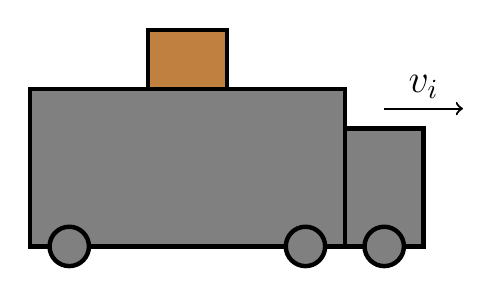
\begin{tikzpicture}
	\filldraw[ultra thick,color=black,fill=gray] (0,0) rectangle (4,2);
	\filldraw[ultra thick,color=black,fill=gray] (4,0) rectangle (5,1.5);
	\filldraw[ultra thick,color=black,fill=gray] (0.5,0) circle (0.25);
	\filldraw[ultra thick,color=black,fill=gray] (3.5,0) circle (0.25);
	\filldraw[ultra thick,color=black,fill=gray] (4.5,0) circle (0.25);
	\filldraw[ultra thick,color=black,fill=brown] (1.5,2) rectangle (2.5,2.75);
	\draw[thick,->] (4.5,1.75) -- (5,1.75) node[anchor=south] {\Large$v_{i}$} -- (5.5,1.75);
\end{tikzpicture}
\end{textblock*}
\newpage
\begin{TeacherMargin}
\begin{center}
	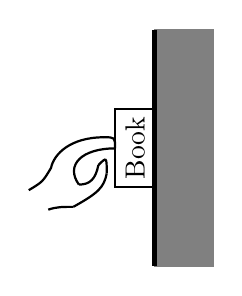
\begin{tikzpicture}
		\filldraw[gray] (0,-1.5) rectangle (0.75,1.5);
		\draw[ultra thick] (0,1.5) -- (0,-1.5);
		\draw[thick] (-0.5,-0.5) rectangle (0,0.5);
		\node[rotate=90] at (-0.25,0) {Book};
		\begin{scope}[shift={(-1.28,-0.5)},rotate=45]
			\draw[thick] (-0.25,0.2) .. controls (-0.05,0.15) .. (0.15,0.2) .. controls (0.3,0.3) and (0.6,0.3) .. (0.9,0);
			\draw[thick] (0.9,0) .. controls (1,-0.1) .. (0.9,-0.2);
			\draw[thick,shift={(0,-0.2)}] (0.25,0) .. controls (0.3,0.3) and (0.6,0.3) .. (0.9,0);
			\draw[thick] (0.25,-0.2) .. controls (0.35,-0.3) and (0.45,-0.3) .. (0.6,-0.2);
			\draw[thick] (0.6,-0.2) .. controls (0.75,-0.2) .. (0.6,-0.35);% -- (0.55,-0.3) -- cycle;
			\draw[thick,shift={(0,-0.15)}] (0,-0.2) .. controls (0.35,-0.3) and (0.45,-0.3) .. (0.6,-0.2);
			\draw[thick,shift={(0,-0.35)}] (-0.25,0.2) .. controls (-0.15,0.15) and (-0.1,0.1) .. (0,0);
		\end{scope}
	\end{tikzpicture}
\end{center}
We have the long-range force of gravity $\vec{F}^{g}_{BE}$ (pointing down), plus forces from two contact interactions:
\begin{itemize}
	\item Hand
	\begin{itemize}
		\item The hand exerts a normal force $\vec{F}^{N}_{BH}$ perpendicular to the cover of the book (pointing right) and a force of static friction $\vec{F}^{sf}_{BH}$ (because it is not sliding along the cover) parallel to the surface of the book.
	\end{itemize}
	\item Wall
	\begin{itemize}
		\item The wall exerts a normal force $\vec{F}^{N}_{BW}$ perpendicular to the cover of the book (pointing left) and a force of static friction $\vec{F}^{sf}_{BW}$ (because the book is not sliding along the wall) parallel to the surface of the book.
	\end{itemize}
\end{itemize}
Both forces of static friction point upward to prevent the downward motion that would otherwise occur.
\begin{center}
	\begin{tikzpicture}
		\FBDaxes{0,0}{0}{axes}
		\FBDbox[0.6]{axes}{0}{box}{}
		\FBDvectorXY{boxtlq}{0,1}{FSH}
		\node[anchor=east] at (FSHtip) {$\vec{F}^{sf}_{BH}$};
		\FBDvectorXY{boxtrq}{0,0.5}{FSW}
		\node[anchor=west] at (FSWtip) {$\vec{F}^{sf}_{BW}$};
		\FBDvectorXY{boxbcent}{0,-1.5}{FG}
		\node[anchor=east] at (FGtip) {$\vec{F}^{g}_{BE}$};
		\FBDvectorXY{boxrcent}{1.25,0}{FNH}
		\node[anchor=south] at (FNHtip) {$\vec{F}^{N}_{BH}$};
		\FBDvectorXY{boxlcent}{-1.25,0}{FNW}
		\node[anchor=south] at (FNWtip) {$\vec{F}^{N}_{BW}$};
	\end{tikzpicture}
\end{center}
To keep $F^{net}_{x} = 0$, we must have $F^{N}_{BH} = F^{N}_{BW}$. \\
To keep $F^{net}_{y}=0$, we need $F^{g}_{BE} = F^{sf}_{BH} + F^{sf}_{BW}$. \\
For static friction, we know $F^{sf}\leq\mu_{s}F^{N}$, so we can find the maximum possible static frictions, but that does not tell us what $F^{sf}_{BH}$ and $F^{sf}_{BW}$ are exactly. We don't even know if they are equal to each other (so I gave them two different arbitrary lengths in my FBD). \\

\noindent\textbf{Pushing Harder}
\begin{itemize}
	\item $F^{g}=mg$, so it will remain constant.
	\item $F^{N}_{BH}$ is the push, and $F^{N}_{BW} = F^{N}_{BH}$, so both must increase.
	\item $F^{sf}_{BH}+F^{sf}_{BW} = F^{g}_{BE}$, so $F^{sf}_{BH}+F^{sf}_{BW}$ is constant, but we don't really know about $F^{sf}_{BH}$ and $F^{sf}_{BW}$ individually.
\end{itemize}
\end{TeacherMargin}
\begin{PresentSpace}
\vspace{-10pt}
\section*{L\Week-1: Book on the Wall -- Hold Still}
\vspace{-10pt}
\begin{itemize}
	\item You push a book against a vertical wall so the book does not move.
	\begin{itemize}
		\item Sketch a picture of the book and the wall.
		\item Identify and describe each force acting on the book.
		\item Draw and label a free-body diagram for the book.
	\end{itemize}
	\item What do you know about the magnitudes of the forces acting on the book?
	\item What happens to each force if you push harder?
\end{itemize}
\end{PresentSpace}
\newpage
\begin{TeacherMargin}
\noindent\textbf{Differences} \\
We have one less force of friction, and the remaining friction is now kinetic. It still points up, as it opposes the downward motion along the wall.
\begin{center}
	\begin{tikzpicture}
		\FBDaxes{0,0}{0}{axes}
		\FBDbox[0.6]{axes}{0}{box}{}
		%\FBDvectorXY{boxtlq}{0,1}{FSH}
		%\node[anchor=east] at (FSHtip) {$\vec{F}^{sf}_{BH}$};
		\FBDvectorXY{boxtcent}{0,1.5}{FKW}
		\node[anchor=west] at (FKWtip) {$\vec{F}^{kf}_{BW}$};
		\FBDvectorXY{boxbcent}{0,-1.5}{FG}
		\node[anchor=east] at (FGtip) {$\vec{F}^{g}_{BE}$};
		\FBDvectorXY{boxrcent}{1.25,0}{FNH}
		\node[anchor=south] at (FNHtip) {$\vec{F}^{N}_{BH}$};
		\FBDvectorXY{boxlcent}{-1.25,0}{FNW}
		\node[anchor=south] at (FNWtip) {$\vec{F}^{N}_{BW}$};
	\end{tikzpicture}
\end{center}
Speed is constant, so net force is still zero, and now we have an equality relating friction to the normal force: $F^{kf}_{BW} = \mu_{bw}F^{N}_{BW}$.  We can use this to solve for the required normal force.
\begin{align*}
	F^{net}_{x} & = F^{N}_{BH}-F^{N}_{BW} = 0 & F^{net}_{y} & = F^{kf}_{BW} - F^{g}_{BE} = 0 \\
	& \implies F^{N}_{BH} = F^{N}_{BW} & & \implies F^{kf}_{BW} = F^{g}_{BE} \\
	& & & \implies \mu_{bw}F^{N}_{BW} = mg \\
	& & & \implies \mu_{bw}F^{N}_{BH} = mg
\end{align*}
The hand must exert a force of magnitude $F^{N}_{BH} = \frac{mg}{\mu_{bw}}$. \\

\noindent\textbf{Unit check} \\
We know $F^{N}_{BH}$ is a force, so its units are newtons. Therefore, we need $\frac{mg}{\mu_{bw}}$ to also be a force. We already know $mg$ has the proper units, and coefficients of friction are unitless, so $\frac{mg}{\mu_{bw}}$ is indeed a force. \\
\textbf{Covariation}
\begin{itemize}
	\item If the book gets heavier ($m$ increases, or we do this on a planet with larger $g$ than Earth), then we should expect it to be harder to support.
	\begin{itemize}
		\item $F^{N}=\frac{mg}{\mu_{bw}}$, so if $mg$ increases, $F^{N}_{BH}$ increases, as we expect.
	\end{itemize}
	\item If the wall gets rougher or grippier ($\mu_{bw}$ increases), then it should be easier to keep the book from falling faster.
	\begin{itemize}
		\item $F^{N}=\frac{mg}{\mu_{bw}}$, so if $\mu_{bw}$ increases, $F^{N}_{BH}$ decreases, as we expect.
	\end{itemize}
\end{itemize}
\textbf{Special Case} \\
If the wall is frictionless ($\mu_{bw}=0$), then nothing will keep the book from accelerating downward, so it is impossible to push it hard enough. \\
From our equation, $F^{N}_{BH} = \frac{mg}{0} = \infty$. Infinite force is impossible, so the equation is telling us what we expect.
\end{TeacherMargin}
\begin{PresentSpace}
\vspace{-10pt}
\section*{L\Week-2: Book on the Wall -- Slide Down}
\vspace{-10pt}
\begin{itemize}
	\item You push a different book horizontally against a vertical wall so that the book slides downward at constant speed.
	\item You know the coefficients of friction are $\mu_{bw}$ (between the book and the wall) and \textit{zero} (between the book and your hand). You also know the mass $m$ of the book.
	\begin{itemize}
		\item Draw a free-body diagram for this situation.
		\item Determine the magnitude of the force that your hand must exert on the book.
		\item Make sense of your answer in at least three different ways.
	\end{itemize}
\end{itemize}
\end{PresentSpace}
\newpage
\begin{TeacherMargin}
	
\end{TeacherMargin}
\begin{PresentSpace}
\section*{Main Ideas}
\begin{itemize}
	\item There are many different \textit{kinds} of forces that we can analyze differently.
	\item Objects can only change their motion when acted upon by an external force.
	\item The net force on an object is equal to its mass times its acceleration.
	\item Forces are vectors.
	\item When more than one force acts on an object, we can add all the forces together.
	\item We can model forces quantitatively.
	\item When an object is at rest or moving at constant speed, the forces balance and the object is in equilibrium.
\end{itemize}
\end{PresentSpace}
\end{document}